\documentclass{bredelebeamer}
\usepackage[superscript]{cite}
\usepackage[sort&compress,comma,super]{natbib}


\title[Eshmun]{Concurrent Model Repair: Eshmun}
% Titre du diaporama

\subtitle{Models, Repairs, and Formal Verification}
% Sous-titre optionnel

\author{Ali Cherri\inst{1}, Kinan Dak Al Bab\inst{1}}

\institute[AUB]
{
  \inst{1}%
  American University of Beirut\\
  Department of Computer Science
  }


\date{19 May 2015}

\subject{Model Repair}


%%%%%%%%%%%%%%%%%%%%%%%%%%%%%%%%%%%%%%%%%%%%%%%%%%%%%%%%%%%%%%%%%%%%%
\begin{document}

\begin{frame}
  \titlepage
\end{frame}


%%%%%%%%% PART 1: OVERVIEW
\begin{frame}{Getting Started}
  \tableofcontents
\end{frame}

%%%%%%%%% PART 2: MOTIVATION
\section{Why Formal Verification ?}

\begin{frame}{Why Formal Verification ?}
\begin{block}{Computing Catastrophes\citep{bugs}}
\begin{itemize}
\item \alert{Ariane 5}: Blew up due to code re-use without verification.
\item \alert{Therac-25}: Radiation Therapy Machine. Killed 6 due to a software error.
\item \alert{Mars Climate Crasher}: Crashed on Mars after 286-days trip. Due to unit conversions.
\item \alert{AT\&T}: AT\&T assumed it was being hacked. In fact, the company's long distance switches kept rebooting in sequence.

\end{itemize}
\end{block}

\begin{block}{Dijkstra's Thoughts\citep{dijkstra}}
The formal provability of a program is a major criterion for correctness: the central challenges of computing hadn’t been met, due to an insufficient emphasis on program correctness.
\end{block}

\end{frame}

%%%%%%%%% PART 3: Preliminaries
\section{Preliminaries}

\begin{frame}{Modeling Sequential Programs} %SINGLE KRIPKE
\begin{tabular}{l r}
\begin{minipage}{0.5\textwidth}
\vspace{-5mm}
\hspace{-5mm}
\noindent {\large Kripke Structure:}
\begin{itemize}
\item State-transition Diagram: A Directed Graph where nodes are states of the program, and edges are transitions.
\item Used to model sequential programs.
\item The full diagram represents all the possible executions of the program.
\item Each state satisfies certain properties (Boolean Formulae).
\end{itemize} 
\end{minipage}
&
\begin{minipage}{0.5\textwidth}
\begin{figure}
\centering
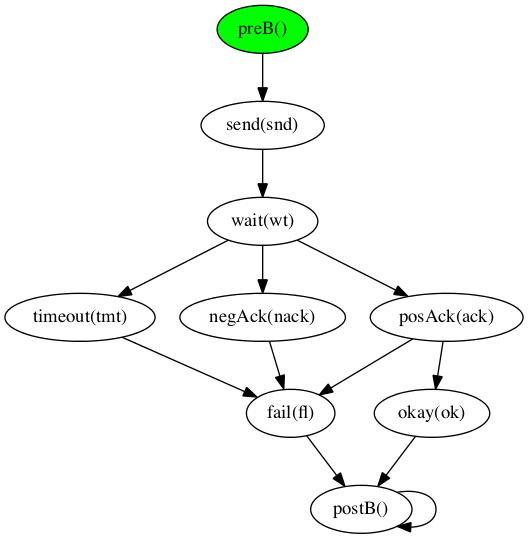
\includegraphics[scale=0.2]{kripke.jpg}
\caption{Kripke Structure for a Phone call}
\end{figure}
\end{minipage}
\end{tabular}
\end{frame}

\begin{frame}{Modeling Asynchronous Concurrent Programs} %MULTI KRIPKE
\begin{tabular}{l r}
\begin{minipage}{0.5\textwidth}
\vspace{-5mm}
\hspace{-5mm}
\noindent {\large Multi-Kripke Structure:}
\begin{itemize}
\item Several Kripke Structure.
\item Each Kripke Structure relates to two processes.
\item Doing things in \emph{pairwise representation} is more efficient!
\end{itemize} 
\end{minipage}
&
\begin{minipage}{0.5\textwidth}
\begin{figure}
\centering
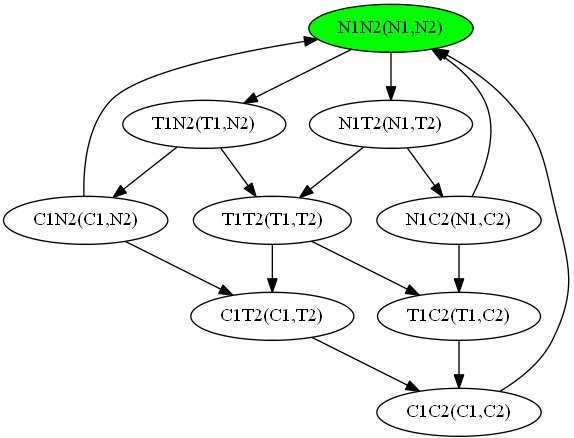
\includegraphics[scale=0.3]{multi.jpg}
\caption{Pair Kripke Structure}
\end{figure}
\end{minipage}
\end{tabular}
\end{frame}

\begin{frame}{Temporal Logic} % TEMPORAL LOGIC
\begin{tabular}{l r}
\begin{minipage}{0.5\textwidth}
\vspace{-5mm}
\hspace{-5mm}
\begin{block}{Definition}
Temporal Logic is a system of rules and boolean propositions that are quantified in terms of time. e.g. I am always Hungry.
\end{block}
\vspace{5mm}
\noindent {\large Computation Tree Logic (CTL)\citep{modelcheck}}
\begin{itemize}
\item Subset of Temporal Logic.
\item Useful in tree-like structures where the future is not determined.
\item Path Operators: quantify over a branch, path, or combination of both.
\item CTL is useful for expressing properties like liveness and safety.
\end{itemize}
\end{minipage}
&
\begin{minipage}{0.5\textwidth}
\begin{figure}
\centering
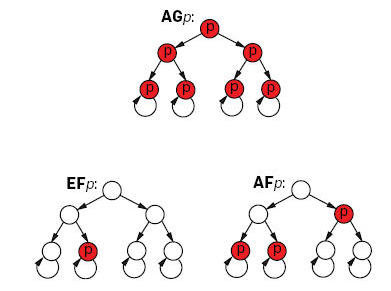
\includegraphics[scale=0.5]{ctl.jpg}
\caption{Notable Temporal Operators}
\end{figure}
\end{minipage}
\end{tabular}
\end{frame}

\begin{frame}{Model Checking\citep{modelcheck}} %Model Checking
\begin{itemize}
\item Used to verify Model Correctness.
\item Given a Model and its Specification (In CTL), determines if the Model satisfies the specs.
\item Great impact on industry:
\begin{itemize}
    \item Used extensivly to verify correctness of Hardware.
    \item Increasing use in verifying correctness of Software (\emph{Windows Device Drivers}).
\end{itemize}
\end{itemize}

\begin{block}{}
Emerson, Clarke, and Sifakis were given the \emph{Turing Award} in 2007 for inventing model checking.
\end{block}
\end{frame}

%%%%%%%% PART 4: PROBLEM & SOLUTION
\section{Defining the Problem: Model Repair} % Problem

\begin{frame}{Model Repair} 
\begin{itemize}
\item We are given a Model and its specifications, the model doesn't satisfy the specifications.
\item We want to apply a \emph{Subtractive Model Repair Algorithm} in order to get a new model that satisfies the specifications.
\item This requires us to find the un-wanted transitions/states that are causing the model to be incorrect.
\item These transitions/states should be \emph{deleted} in a way that doesn't affect the program's flow and totality.
\item The decision version of the problem is proved to be NP-Complete\citep{paper}.
\end{itemize}
\end{frame}

\begin{frame}{Model Repair: The Solution}  % Repair Formula
\begin{itemize}
\item We encode the problem as a boolean formula.
\item The formula contains different types of variables.
\item The value of each variable indicates whether the corresponding state (or transition) is kept or deleted in the new model.
\item The formula forces the new model to be total and have some start state, it also relates States to transitions.
\item The formula is then passed to a SAT solver, each satisfying assignment would represent a repaired model.
\item The Overall length of the repair formula is \emph{$O(|States|^2 \times |Specifications| \times Out\_degree + |States| \times |Transitions| \times |Propositions|)$}\citep{paper}.
\end{itemize}
\end{frame}
\begin{frame}{Model Repair: Getting the New Model } % SAT
\vspace{-5mm}
\hspace{-5mm}
\begin{block}{Boolean Satisfiability Problem (SAT)}
Determining If a boolean formula is Satisfiable or not. Is there an assignment that makes the formula true? Boolean SAT is NP-Complete
\end{block}
\vspace{5mm}
\noindent {\large Repairing with SAT Solver}
\begin{itemize}
\item By construction, if the repair formula is unsatisfiable then the model is un-repairable.
\item Furthermore, the satisfying assignment of the formula is the needed repair.
\item The satisfying assignment tells us which transitions and states are to be deleted.
\item If all the start states are deleted then the model is un-repairable.
\end{itemize}
\end{frame}

%%%%%%%%% PART 5: OUR WORK
\section{Our Work} % Problem
\begin{frame}{What was already done}
\begin{tabular}{l r}
\begin{minipage}{0.5\textwidth}
\begin{itemize}
\item A tool that repairs Single Kripke was done by M. Sakr (master's thesis).
\item The tool used a Model Checker written by Emile Chartouni.
\item The tool was a proof of concept.
\item The tool had techniques that allow you to reduce the model into a smaller one to make repair more efficient.
\item Repairing Mutual Execlusion for 4 Processes required more than 12GB of RAM.
\item Data structures for models and repair algorithm were impossible to extend.
\end{itemize}
\end{minipage}
&
\begin{minipage}{0.5\textwidth}
\begin{figure}
\centering
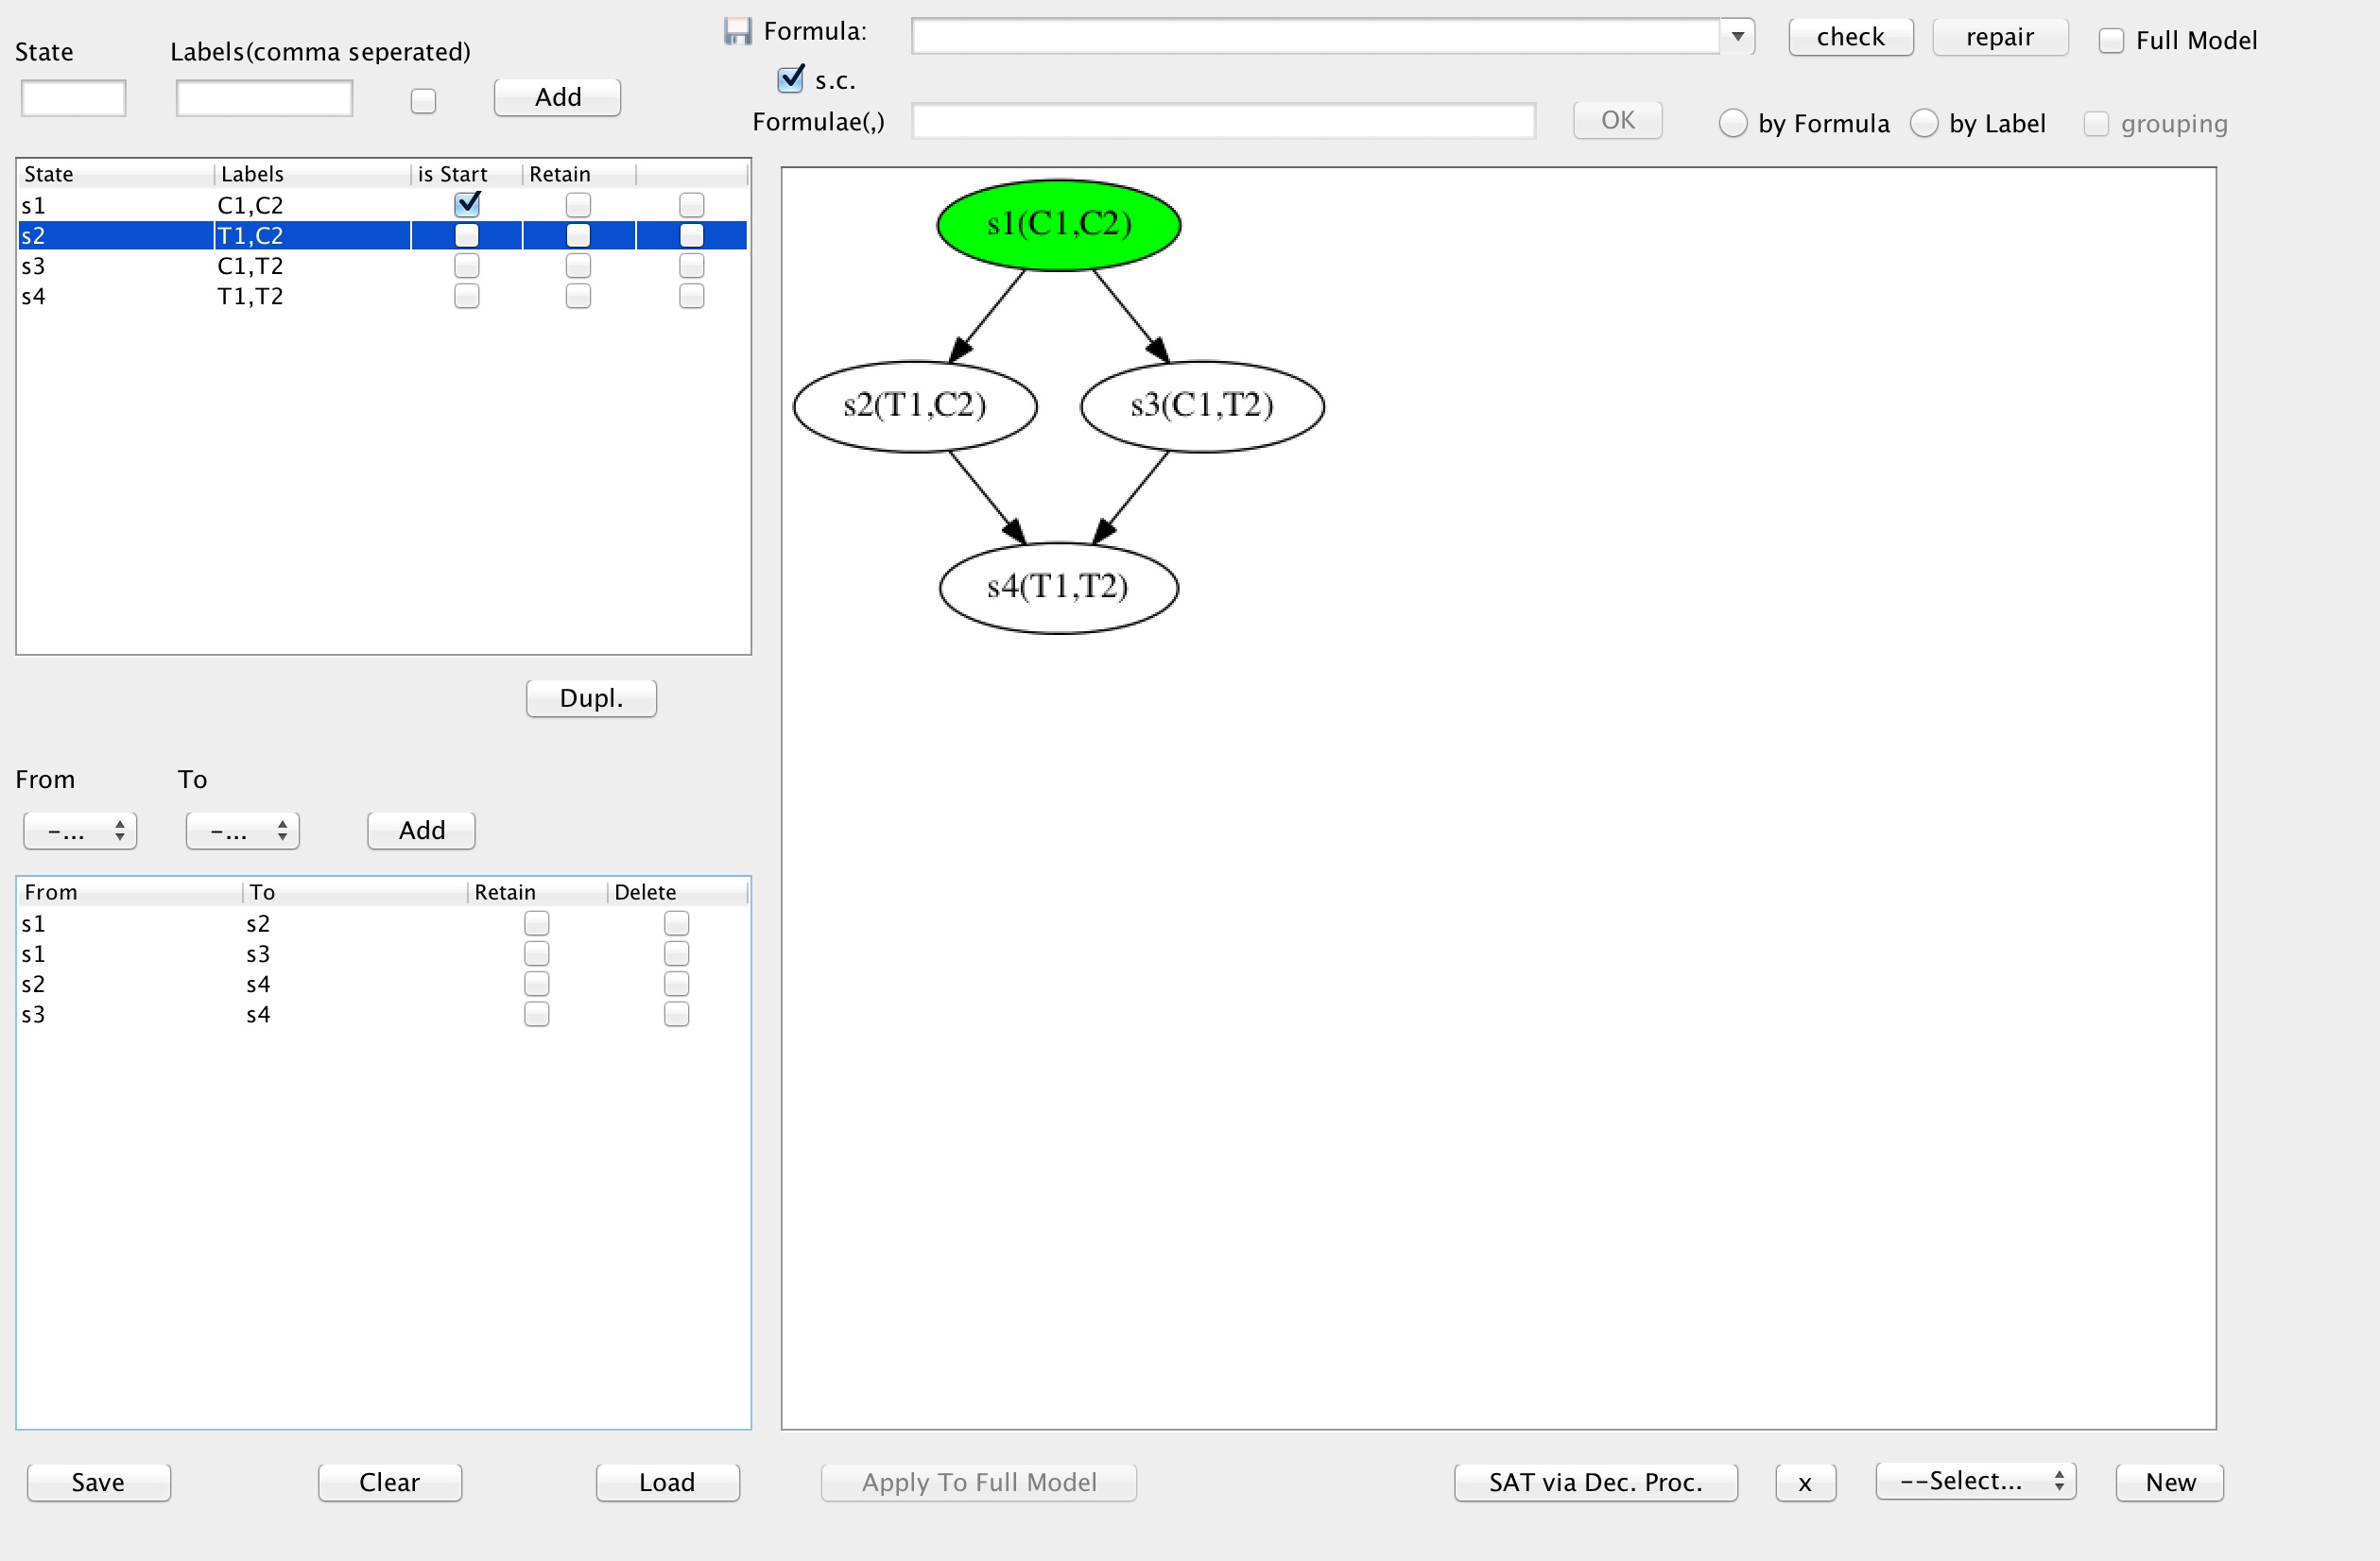
\includegraphics[scale=0.13]{old.png}
\caption{The old tool}
\end{figure}
\end{minipage}
\end{tabular}
\end{frame}

\begin{frame}{Our Contribution: Optimizing the tool}
\begin{itemize}
\item Portability: The previous tool only ran on windows.
\item An easy to use, interactive, and \emph{User Focused} GUI.
\item Feeding the SAT Solver from memory using a custom InputStream.
\item The ability to iterate through different repairs.
\item An IDE like enviroment for inputing Boolean Formulae.
\item Memory Optimization, Implemented a different CTL-Logic API.
\item New Data structures for models, Respecting OOP Guide lines.
\item Complete seperation of modules, each functionality has its own classes in its own packages.
\item Porting the Model Checker and Model Repair to use the new Logic API and datastructures.
\item We re-implemented Everything!!
\end{itemize}
\end{frame}

\begin{frame}{Our Contribution: Multi Kripke Repair}
\begin{itemize}
\item The ability to repair concurrent programs, modeled as Multi-Kripke Structures \emph{Breakthrough}.
\item Each of the sub-kripke structure has its own repair formula.
\item All the sub-repair formulae are conjucted. 
\item A formula for synchronizing the processes across different sub-structures is automatically inferred and added to the complete repair formula.
\end{itemize}
\end{frame}

%%%%%%%%% PART 5: TECHNICAL DETAILS
\section{Technical Details} 

\begin{frame}{Logic API} % LOGIC API
\begin{figure}
\centering
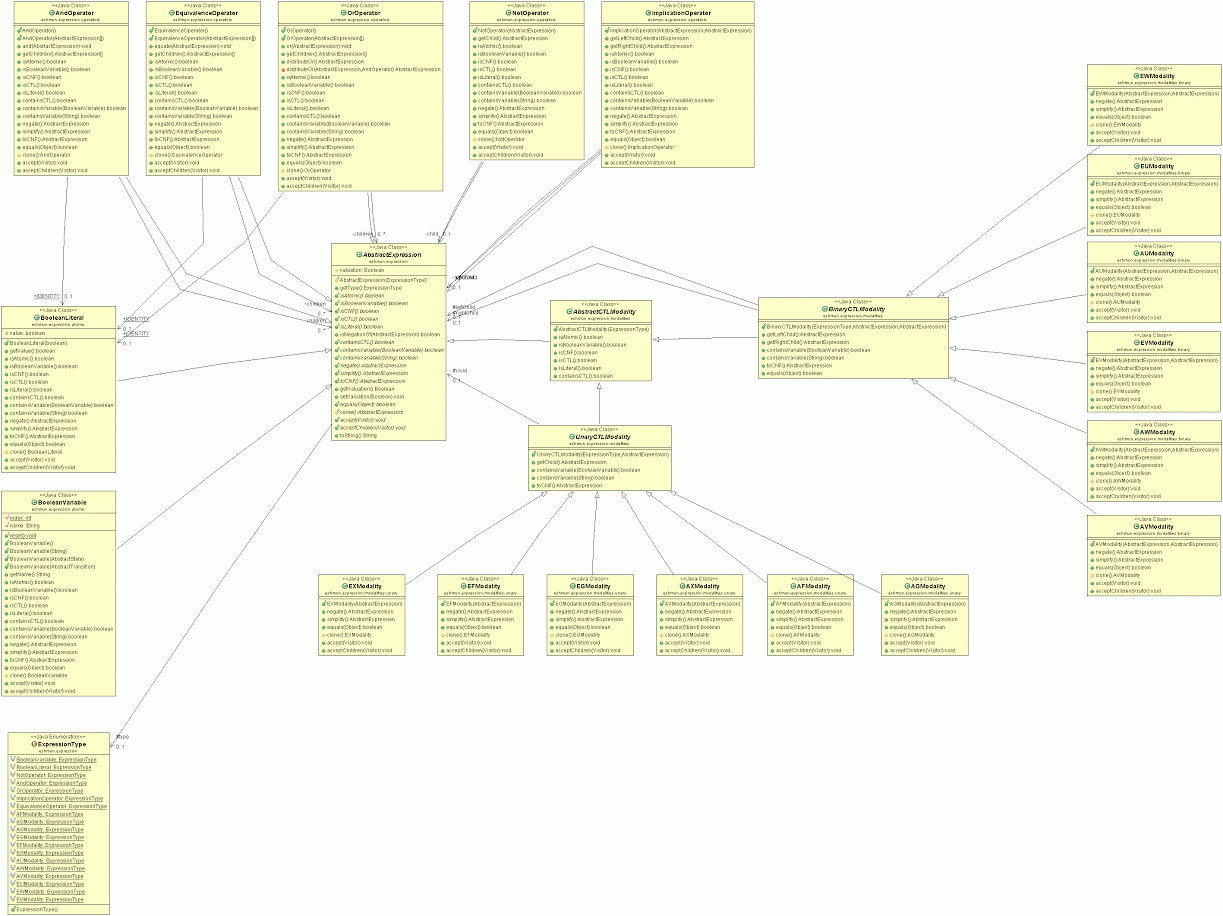
\includegraphics[scale=0.25]{logic.jpg}
\caption{Pair Kripke Structure}
\end{figure}
\end{frame}

\begin{frame}{Data Structures} % DATA STRUCTURES
\begin{figure}
\centering
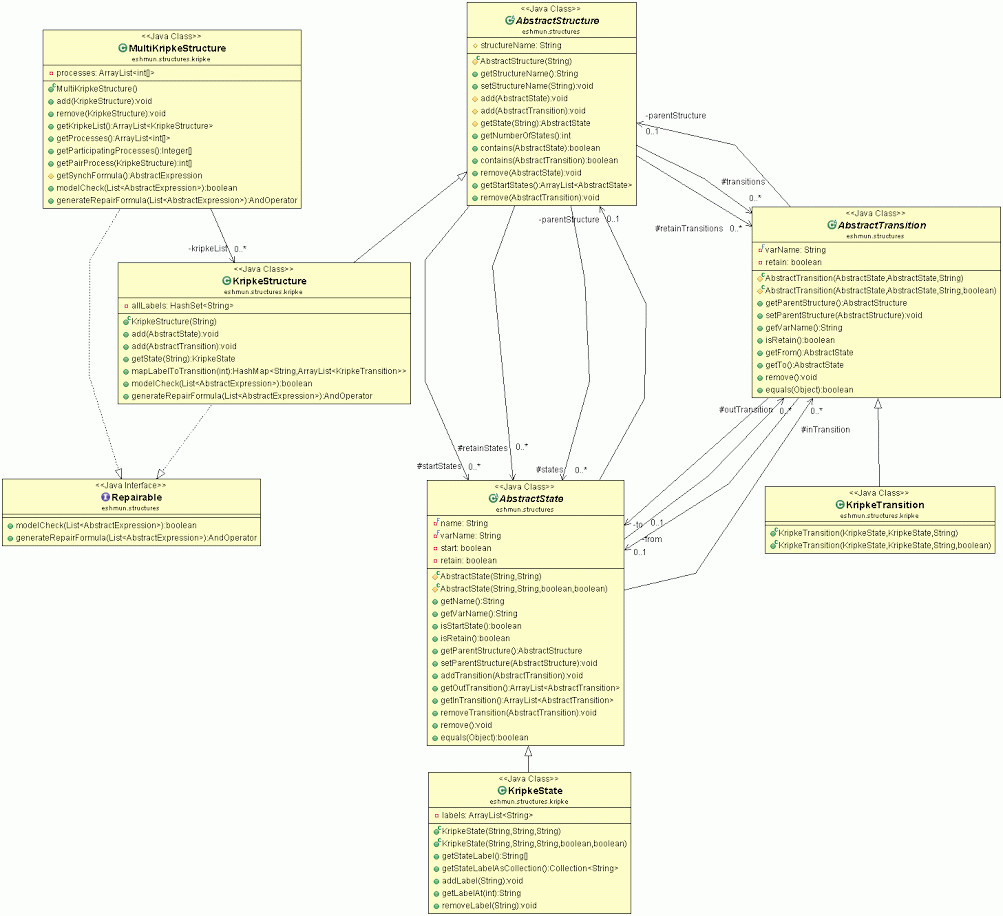
\includegraphics[scale=0.25]{structures.jpg}
\caption{Pair Kripke Structure}
\end{figure}
\end{frame}

\begin{frame}{Some Bragging} % BRAGGING
\begin{block}{Meterics}
\begin{itemize}
\item Number of classes and interfaces: 88
\item Number of methods: 1,027
\item Lines of code: 19,103
\end{itemize}
\end{block}

\begin{block}{Technologies Used}
\begin{itemize}
\item Java : The tool is written in java, it uses extensively concepts from OOP.
\item Java Swing and Graphics2D: used to develop the GUI and the graphics.
\item ANTLR : for building a parser for CTL logic expressions.
\item SAT4J : a sat solver for java.
\item PYTHON: For writting testing scripts, and generating different models.
\item JavaDoc : A complete and extensive documentation of the code is provided.
\item HTML  : Used in the documentation and in the user manuel.
\end{itemize}
\end{block}
\end{frame}

\begin{frame}{Benchmarks} % Benchmarks
\begin{block}{Mutual Exclusion}
\begin{itemize}
\item 2 Process: 107MS --- 93MS
\item 3 Process: 104MS --- 1,210MS
\item 4 Process: 248MS --- Out of Memory
\end{itemize}
\end{block}

\begin{block}{Barrier Synchronization}
\begin{itemize}
\item 2 Process: 63MS ---- 67MS
\item 3 Process: 107MS --- 460MS 
\item 4 Process: 164MS --- 1.1Second
\end{itemize}
\end{block}

\begin{block}{}
These numbers result from repairing the given problems using a single Kripke Structure.
\end{block}
\end{frame}

\section{Future Work} % Future Work

\begin{frame}{Future Work}
\vspace{-5mm}
\hspace{-5mm}
\begin{itemize}
\item Get it published.
\item Support more Concurrent Models: I/O Automata, BIP.
\item Extend to Infinite State Models.
\item Addative Repair Algorithm: add new transitions and states.
\end{itemize}
\end{frame}

\begin{frame}{Credits}
\begin{block}{Credits}
\begin{itemize}
\item We would like to thank our advisor Dr. Paul Attie, he offered a lot of help and guiding.
\item We would like to thank Mohammad Ali Baydoun and George E. Zakhour for providing us with an algorithm 
and a working routine to auto space and format a graph, this was done by simulating the graph as a physical 
system with attraction and repulsion forces.
\end{itemize}
\end{block}
\end{frame}

\section{Conclusion} % Conclusion

\begin{frame}{Summary}
\vspace{-5mm}
\hspace{-5mm}
\begin{itemize}
\item We can Model behavior of programs using formal tools (Kripke, Multi-Kripke, ...).
\item Temporal Logic is an extension of First order logic that is useful to quantify over time (execution paths in case of CTL).
\item By using model checking we can know if a program satisfies a given specification (CTL Formula).
\item We can also Generate a repair formula for the model based on the definition of temporal operators.
\item Using a SAT Solver we can get a satisfying assignment (if it exists) which is by construction the repair formula.
\item We have implemented a tool that does all that.
\end{itemize}
\end{frame}

\begin{frame}
\frametitle{References}

\begin{thebibliography}{9}

\bibitem{bugs}
  \small{Computer World
  \emph{``Infamous 11 software Bugs''}.
  http://www.computerworld.com/article/2515483/enterprise-applications/epic-failures--11-infamous-software-bugs.html?page=4
  }

\bibitem{dijkstra}
  \small{Dijkstra, Edsger W. \emph{``On the Cruelty of Really Teaching Computing Science''}. E.W. Dijkstra Archive. Center for American History, University of Texas at Austin.
  }
  
\bibitem{ioautomata}
  \small{Lynch, Nancy A.; Tuttle, Mark R. (August 1987). \emph{``Hierarchical correctness proofs for distributed algorithms''}. Proceedings of the sixth annual ACM Symposium on Principles of distributed computing. PODC '87
  }
  
\bibitem{modelcheck}
  \small{Pelanek, Radek. \emph{``Formal Verication, Model Checking''}, Talk in ``investice do rozvoje vzdělávání''. http://www.fi.muni.cz/~xpelanek/IA158/slides/verification.pdf
  
  }
  
\bibitem{paper}
  \small{Attie, Paul. Sakr, Mouhammad Issam. (2014). \emph{``Model Repair Via SAT Solving''}. Thesis. M.S. American University of Beirut. Department of Computer Science, 2014. T:6108
  }
  
\end{thebibliography}

\end{frame}

\begin{frame}{Conclusion}

\pgftext[at=\pgfpoint{.43\paperwidth}{0},center,center]{\Huge\structure{Thank You}}

\end{frame}

\end{document}
